\chapter{Elements}\label{ch:Elements}
\begin{chapter_resume}
Este capítulo contiene ejemplos de como realizar las principales acciones necesarias para redactar un documento, y con especial énfasis, una tesis.

\vspace{0.7cm}

Es conveniente recordar que es útil tener un capítulo que incluya los principales elementos, ya que es útil para asegurar la correcta compilación de todos los paquetes. 
Es decir, tener siempre un capítulo que incluya una referencia, un acrónimo, un símbolo, una tabla y una figura y utiliza todos la mayoría de los paquetes por lo que nos permite chequear que el documento está correctamente diseñado en todo momento sin ralentizar la compilación de este.

\vspace{0.7cm}

Sin más, sólo recordar que para reproducir cualquier utilidad aquí mostrada no hay más que copiar el código fuente y pegarlo en el lugar deseado del documento. Se incluye un resumen de los diferentes códigos sin explicación en el siguiente capítulo
\end{chapter_resume}
En este capítulo se dividen por secciones lo principales elementos a incorporar en un documento. En cada sección se muestran las distintas posibilidades que se ofrecen para insertar nuevos elementos así como comentarios acerca de su uso, limitaciones o precauciones.
\section{Figures}\label{sec:Elements_figures}
%\begin{figure}[ht]
%\centering
%\includesvg[scale=0.5]{svgimage}
%\caption{A svg image example}
%\label{fig:x cubedvv graph}
%\end{figure}
\begin{lstlisting}
\begin{figure}[h]
\centering
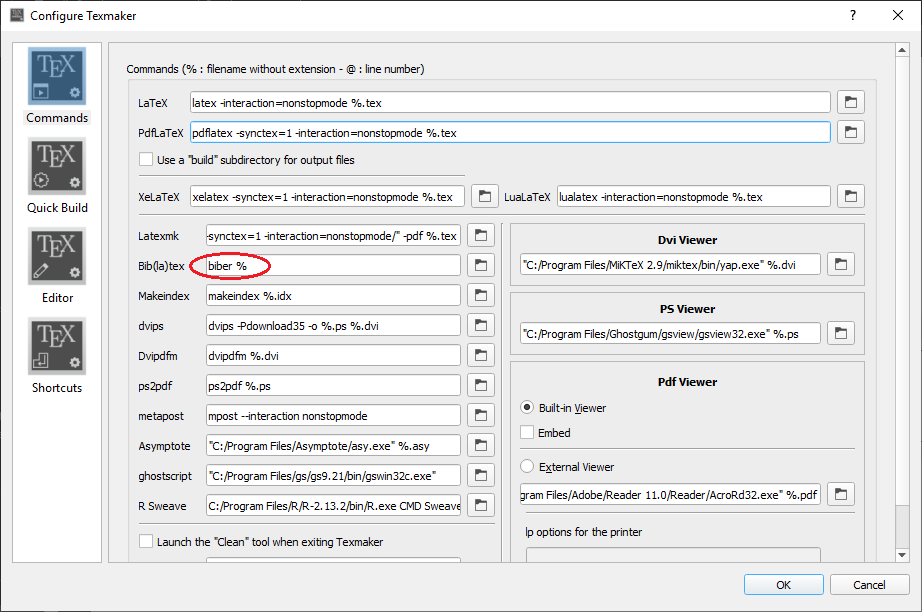
\includegraphics[width=.45\textwidth]{Intro_TexMakerConf.png}
\caption[Resume line]{An example graph}
\label{fig:example}
\end{figure}
\end{lstlisting}

\begin{figure}[h]
\centering
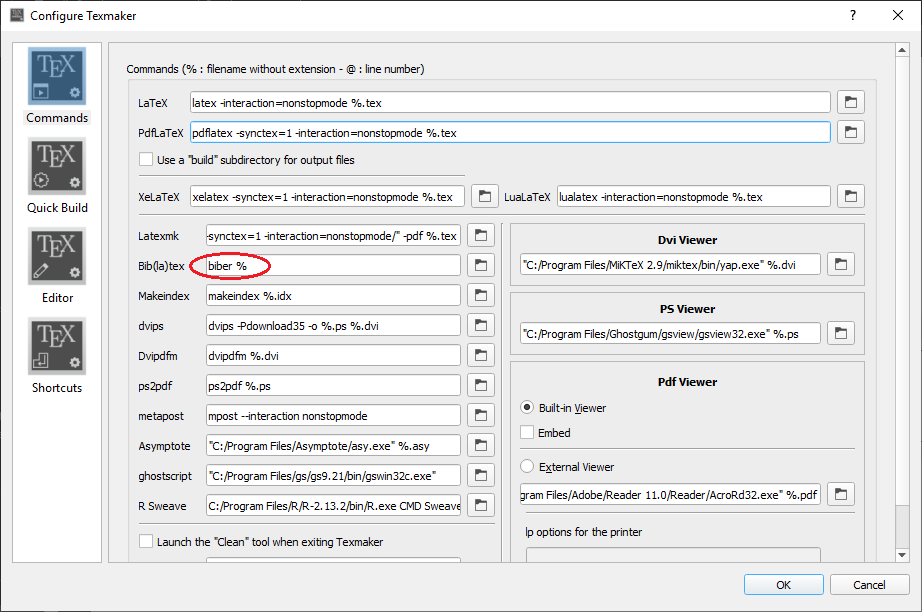
\includegraphics[width=.45\textwidth]{Intro_TexMakerConf.png}
\caption[Resume line]{An example graph}
\label{fig:example}
\end{figure}

\begin{lstlisting}
\begin{figure}[h]
    \centering
    \begin{subfigure}[b]{.3\textwidth}
        \centering
        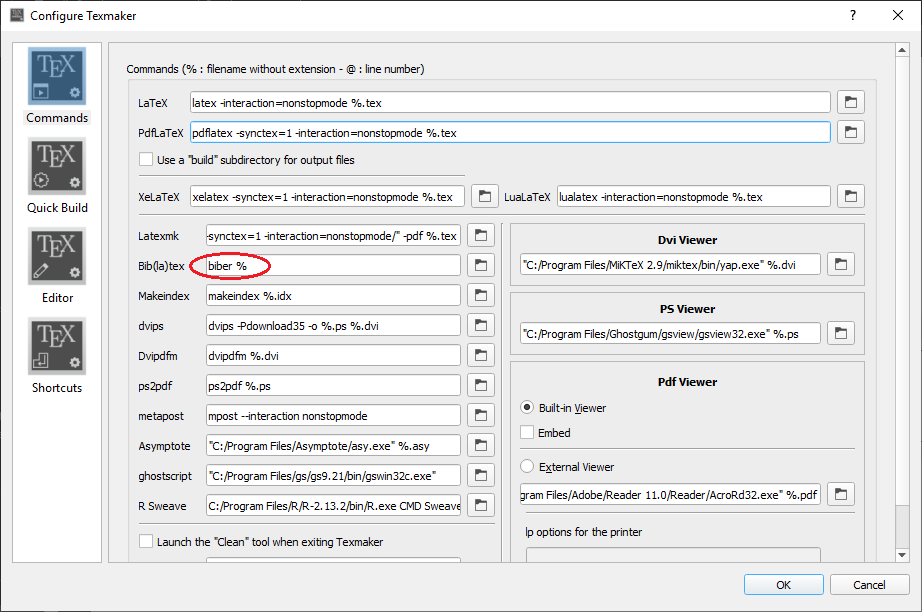
\includegraphics[width=\textwidth]{Intro_TexMakerConf.png}
        \caption{$y=x$}
        \label{fig:triple_x}
    \end{subfigure}
    \hfill
    \begin{subfigure}[b]{0.3\textwidth}
        \centering
        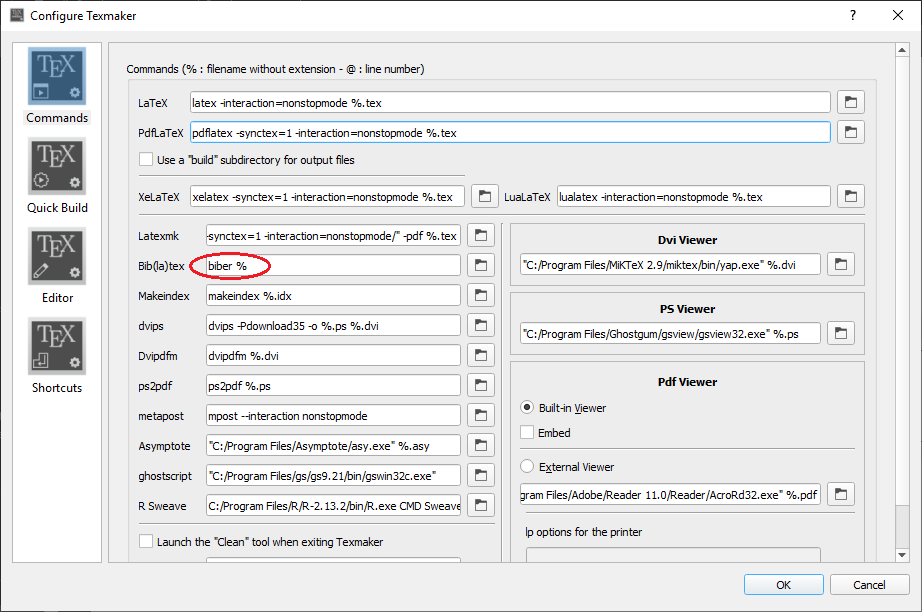
\includegraphics[width=\textwidth]{Intro_TexMakerConf.png}
        \caption{$y=3sinx$}
        \label{fig:triple_3sinx}
    \end{subfigure}
    \hfill
    \begin{subfigure}[b]{0.3\textwidth}
        \centering
        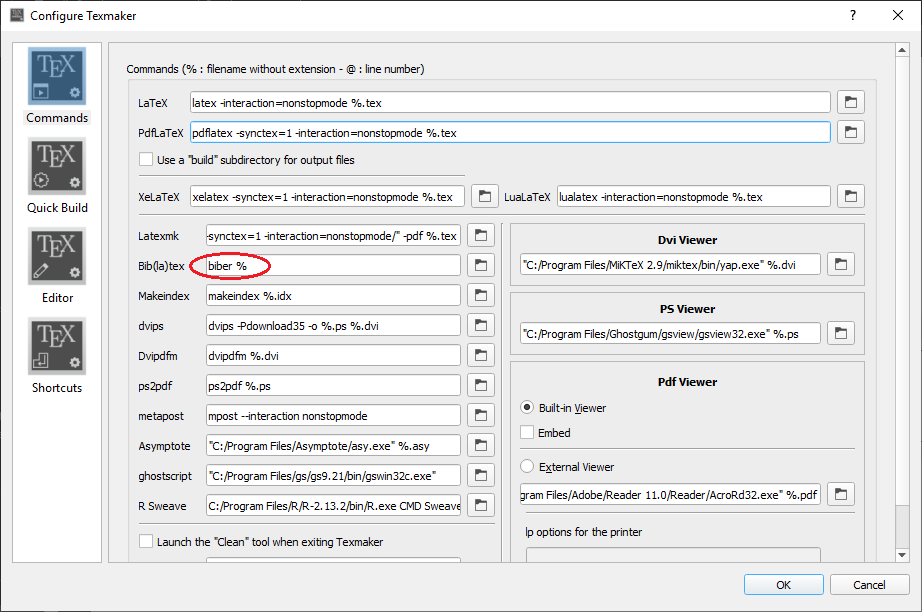
\includegraphics[width=\textwidth]{Intro_TexMakerConf.png}
        \caption{$y=5/x$}
        \label{fig:triple_5overx}
    \end{subfigure}
    \caption[Resume line]{Three simple graphs}
    \label{fig:triple}
\end{figure}
\end{lstlisting}

\begin{figure}[h]
    \centering
    \begin{subfigure}[b]{.3\textwidth}
        \centering
        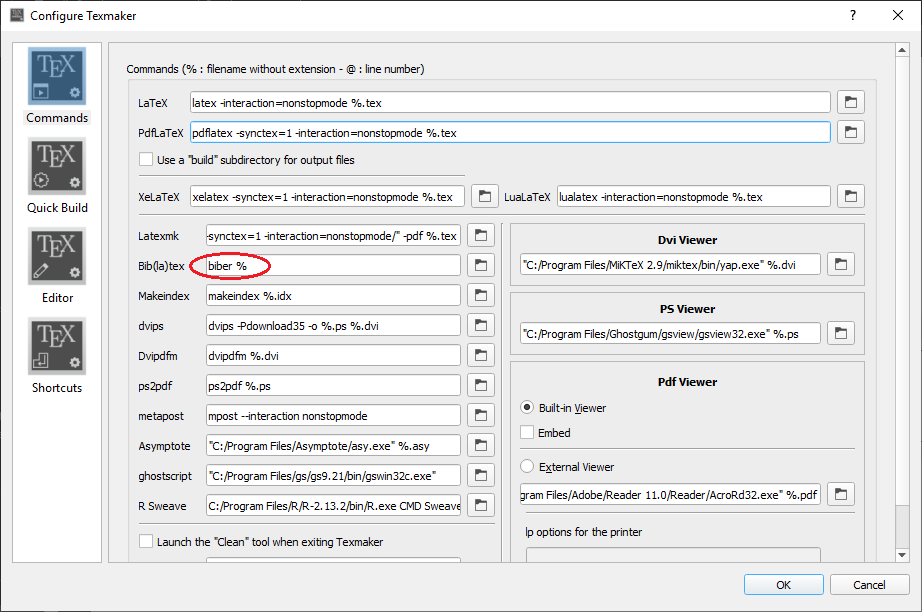
\includegraphics[width=\textwidth]{Intro_TexMakerConf.png}
        \caption{$y=x$}
        \label{fig:triple_x}
    \end{subfigure}
    \hfill
    \begin{subfigure}[b]{0.3\textwidth}
        \centering
        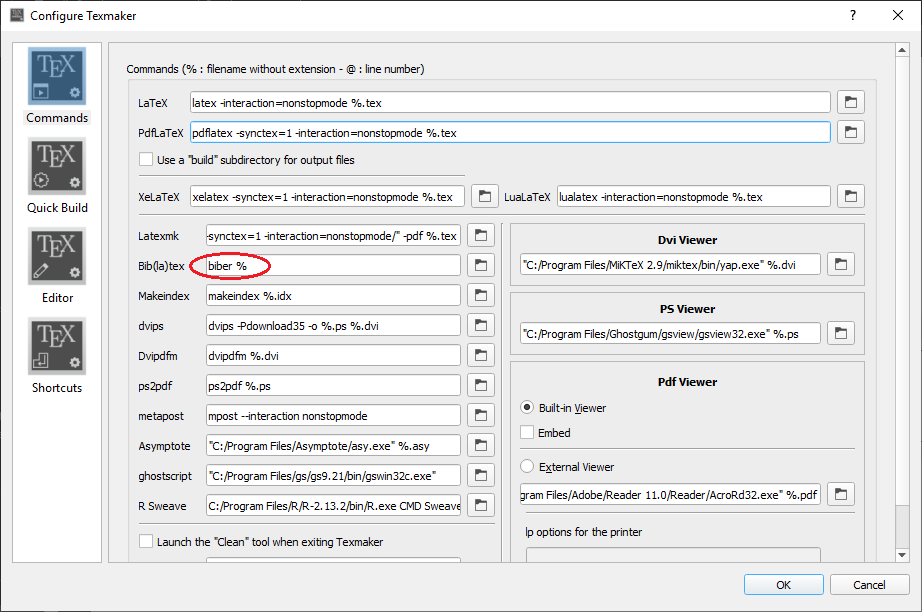
\includegraphics[width=\textwidth]{Intro_TexMakerConf.png}
        \caption{$y=3sinx$}
        \label{fig:triple_3sinx}
    \end{subfigure}
    \hfill
    \begin{subfigure}[b]{0.3\textwidth}
        \centering
        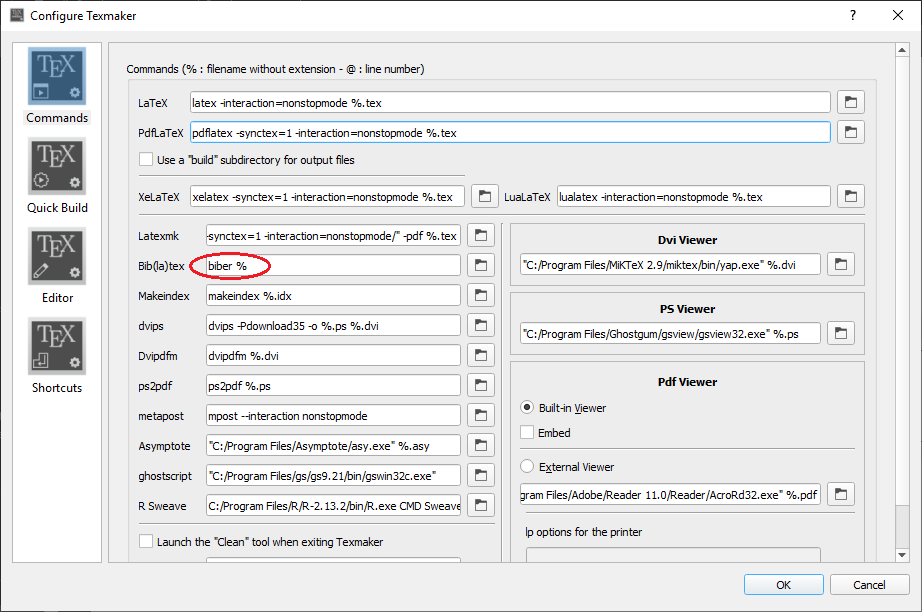
\includegraphics[width=\textwidth]{Intro_TexMakerConf.png}
        \caption{$y=5/x$}
        \label{fig:triple_5overx}
    \end{subfigure}
    \caption[Resume line]{Three simple graphs}
    \label{fig:triple}
\end{figure}
\section{Tables}\label{sec:Elements_tables}

\begin{lstlisting}
\begin{table}[ht]
	\centering
	\begin{tabular}{l | l | l}
	A & B & C \\
	\hline
	1 & 2 & 3 \\
	4 & 5 & 6
	\end{tabular}
	\caption{very basic table}
	\label{tab:example}
\end{table}
\end{lstlisting}

\begin{table}[ht]
	\centering
	\begin{tabular}{l | l | l}
	A & B & C \\
	\hline
	1 & 2 & 3 \\
	4 & 5 & 6
	\end{tabular}
	\caption{very basic table}
	\label{tab:example}
\end{table}
%
%\begin{table}[ht]
%    \begin{subtable}[h]{0.45\textwidth}
%        \centering
%        \begin{tabular}{l | l | l}
%        Day & Max Temp & Min Temp \\
%        \hline \hline
%        Mon & 20 & 13\\
%        Tue & 22 & 14\\
%        Wed & 23 & 12\\
%        Thurs & 25 & 13\\
%        Fri & 18 & 7\\
%        Sat & 15 & 13\\
%        Sun & 20 & 13
%        \end{tabular}
%        \caption{First Week}
%        \label{tab:week1}
%    \end{subtable}
%    \hfill
%    \begin{subtable}[h]{0.45\textwidth}
%        \centering
%        \begin{tabular}{l | c | c}
%        Day & Max Temp & Min Temp \\
%        \hline \hline
%        Mon & 17 & 11\\
%        Tue & 16 & 10\\
%        Wed & 14 & 8\\
%        Thurs & 12 & 5\\
%        Fri & 15 & 7\\
%        Sat & 16 & 12\\
%        Sun & 15 & 9
%        \end{tabular}
%        \caption{Second Week}
%        \label{tab:week2}
%    \end{subtable}
%    \caption{Max and min temps recorded in the first two weeks of July}
%    \label{tab:temps}
%\end{table}
\section{Equations}\label{sec:Elements_equations}
Ecuaciones:

\begin{enumerate}

\item In-line equation:

This is \lstinline"$E=mc^2$" in-line $\rightarrow$ This is $E=mc^2$ in-line

This is \lstinline"$\frac{\frac{1}{x}+\frac{1}{y}}{y-z}$" as well $\rightarrow$ This is $\frac{\frac{1}{x}+\frac{1}{y}}{y-z}$ as well\\

\item Numbered equation:

\begin{lstlisting}
\begin{equation}\label{eq:someequation}
\sqrt[n]{1+x+x^2+x^3+\dots+x^n}
\end{equation}
\end{lstlisting}

\begin{equation}\label{eq:someequation}
\sqrt[n]{1+x+x^2+x^3+\dots+x^n}
\end{equation}

\item Unnumbered equation:

\begin{lstlisting}
\begin{equation*}
\frac{n!}{k!(n-k)!} = \binom{n}{k}
\end{equation*}
\end{lstlisting}

\begin{equation*}
\frac{n!}{k!(n-k)!} = \binom{n}{k}
\end{equation*}
\end{enumerate}
\section{Cites}\label{sec:Elements_cites}
\begin{enumerate}
  \item Cita estándar:
  
  \verb=\cite{Hovel1997b}= $\rightarrow$  \cite{Hovel1997b}
  
  \verb=\cite{Rau2007,King2011}= $\rightarrow$  \cite{King2011,Rau2007}\\
  
  \item Cita comentada:
  
  \verb=\parencite[e.g.][page 300]{Miller2012}= $\rightarrow$ \parencite[e.g.][page 300]{Miller2012}
\end{enumerate}

\section{References}\label{sec:Elements_refs}

\begin{enumerate}
  \item Figure reference:
  
  \verb=\ref{fig:example}= $\rightarrow$ \ref{fig:example}
  
  \verb=\ref{fig:triple}= $\rightarrow$ \ref{fig:triple}\\
  
  \item Subfigure reference:
  
  \verb=\ref{fig:triple_x}= $\rightarrow$ \ref{fig:triple_x}
  
  \verb=\subref{fig:triple_x}= $\rightarrow$ \subref{fig:triple_x}\\
  
  \item Table reference:
  
  \verb=\ref{tab:example}= $\rightarrow$ \ref{tab:example}\\
  
  \item Equation reference:
  
  \verb=\ref{eq:someequation}= $\rightarrow$ \ref{eq:someequation}
  
  \verb=\eqref{eq:someequation}= $\rightarrow$ \eqref{eq:someequation}\\
  
  \item Chapter reference:
  
  \verb=\ref{ch:Elements}= $\rightarrow$ \ref{ch:Elements}
  
  \verb=\nameref{ch:Elements}= $\rightarrow$ \nameref{ch:Elements}\\
  
  \item Section reference:
  
  \verb=\ref{sec:Elements_refs}= $\rightarrow$ \ref{sec:Elements_refs}
  
  \verb=\nameref{sec:Elements_refs}= $\rightarrow$ \nameref{sec:Elements_refs}\\
\end{enumerate}


\section{Acronyms and symbols}\label{sec:Elements_acrosyms}
\begin{enumerate}
  \item Symbol:
  
  \verb=\gls{symbol1}= $\rightarrow$ \gls{symbol1}

  \item Acronym:

  \verb=\gls{acronym1}= $\rightarrow$ \gls{acronym1}
\end{enumerate}
\section{Lists}\label{sec:Elements_lists}
This is a list
\begin{lstlisting}
\begin{enumerate}
  \item First points
  \item Second
  \item Etc
\end{enumerate}
%\end{tabular}
Esto es una lista.
\end{lstlisting}

%\begin{tabular}{p{0.7\textwidth}}
\begin{enumerate}
  \item First points
  \item Second
  \item Etc
\end{enumerate}
%\end{tabular}

This is another list set to start at 8
  
\begin{lstlisting}
\begin{enumerate}
  \setcounter{enumi}{7}	
  \item First points
  \item Second
  \item Etc
\end{enumerate}
%\end{tabular}
Esto es una lista.
\end{lstlisting}

%\begin{tabular}{p{0.7\textwidth}}
\begin{enumerate}
  \setcounter{enumi}{7}
  \item First points
  \item Second
  \item Etc
\end{enumerate}
%\end{tabular}